\documentclass[11pt]{article}
\addtolength{\oddsidemargin}{-1.cm}
\addtolength{\textwidth}{2cm}
\addtolength{\topmargin}{-2cm}
\addtolength{\textheight}{3.5cm}

\usepackage[pdftex]{graphicx}
\usepackage{hyperref}
\usepackage{cite}
\hypersetup{
	colorlinks=true,
	linkcolor=black,
	filecolor=magenta,
	urlcolor=cyan,
}

% define the title
\author{Team CodeX}
\title{Functional Requirements Specification}

\begin{document}
	\setlength{\parskip}{6pt}
	
	% generates the title
	\begin{titlepage}
	
	\begin{center}
		% Upper part of the page       
		
\includegraphics[width=0.7\linewidth]{../Images/eVoting_Logo.png}\\[2cm]    
		\textsc{\LARGE Electronic Voting}\\[0.5cm]
		% Title
		\rule{\linewidth}{0.5mm} \\[1cm]
		{ \huge \bfseries User Manual}\\[0.5cm]
		\rule{\linewidth}{0.5mm} \\[1cm]
		
		% Author and supervisor
<<<<<<< HEAD
		
\includegraphics[width=0.5\linewidth]{../Images/TeamCodexLogo.jpg}\\[0.5cm]    	
=======
		
		
\includegraphics[width=0.5\textwidth]{../Images/TeamCodexLogo.jpg}\\[0.5cm]    	
>>>>>>> 9b25dd959830e00c0e449a84c7623c3e326c347b
		
		
		\begin{minipage}{0.4\textwidth}
			\begin{flushleft} \large
				Andreas {du Preez}
			\end{flushleft}
		\end{minipage}
		\begin{minipage}{0.4\textwidth}
			\begin{flushright} \large
				\emph{} \\
				12207871 
			\end{flushright}
		\end{minipage}
		
		
		\begin{minipage}{0.4\textwidth}
			\begin{flushleft} \large
				\emph{} \\
				Azhar {Mohungoo }
			\end{flushleft}
		\end{minipage}
		\begin{minipage}{0.4\textwidth}
			\begin{flushright} \large
				\emph{} \\
				12239799
			\end{flushright}
		\end{minipage}
		
		
		\begin{minipage}{0.4\textwidth}
			\begin{flushleft} \large
				\emph{} \\
				Gift {Sefako }
			\end{flushleft}
		\end{minipage}
		\begin{minipage}{0.4\textwidth}
			\begin{flushright} \large
				\emph{} \\
				12231097
			\end{flushright}
		\end{minipage}
		
		\textsc{\Large Stakeholders}\\[1cm]	
				
		\begin{minipage}{0.4\textwidth}
			\begin{flushleft} \large
				\emph{} \\
				Epi-Use Advance
			\end{flushleft}
		\end{minipage}
		\begin{minipage}{0.4\textwidth}
			\begin{flushright} \large
				\emph{} \\
				Roelof Nuade
			\end{flushright}
		\end{minipage}
		
	\end{center}
\end{titlepage}
	
	\renewcommand{\thesection}{\arabic{section}}
	\newpage
	
	\tableofcontents
	
	\textsc{}\\[1cm]
	
	\newpage
	
	\section{Introduction}
		This document aims to specify the functional and non-functional requirements as well as the architectural requirements for an electronic voting system specified by CodeX and the client EpiUse.

It will serve as a means of communication between the client and developers as well as providing an elaboration and a clear description of its implementation specifications.
	
	\section{Vision}
		What is intended for this project is to create a web and mobile platform, which can be used to cast votes in the provincial and national elections of South Africa. The following are benefits of the system:
	
	\begin{enumerate}
		\item The use of the Blockchain will allow for a transparent election process while still maintaining anonymity of the voters. 
		\item Votes that get lost or disgarded be it on purpose or not.
		\item Incorrect counting.
		\item Manual vote counting will no longer be required
		\item Remote casting of votes from a users preferred web browser or mobile smartphone. 
		\item Secure voting
		\item Prevent invalid votes from being cast through robust validation with each request.
	\end{enumerate}
	
	\section{Background}
		Elections are always a time where emotions are at a high and passion for a leader has never been greater. Sometimes this emotion and passion for a leader can lead to unlawful activities to get their chosen leader to to win the elections. By moving the system to an electronic environment it removes almost, if not all, these possibilities for unlawful activities to take place by using computers instead of humans. Although with the use of the Blockchain implementation, these activities can be suppressed.
	
Additionally to a secure and safe voting environment that allows ease of access from the voter's mobile or web browser, it will also make the voting process more efficient, with shorter queues to cast a vote and the progress of elections and the final result will be presented more rapidly, with periodic updates as the system analyses these votes. This system can be used in multiple scenarios not only in election. 

A more generic version of the electronic voting system can be implemented to allow users to partake in surveys, where instead of an election poll, users can create their own custom polls in which they can control participation. A further instance would be using such a system for national wide statistics, gathered by completing a poll of some kind, where anonymity is vital.
		
	\section{Functional Requirements}
	
	\subsection{Use Case Prioritization}
		\input{UseCasePrioritization.tex}
	
	\subsection{Service Contracts}
	\input{ServiceContracts.tex}
	
	\subsection{Required Functionality}
	\input{RequiredFunctionality.tex}
	
	\subsection{Process Specifications}
	\input{ProcessSpecifications.tex}
	
	\subsection{Domain Model}
	\begin{enumerate}
		\item \textbf{Voter}
			\begin{figure}[H]
				\centering
				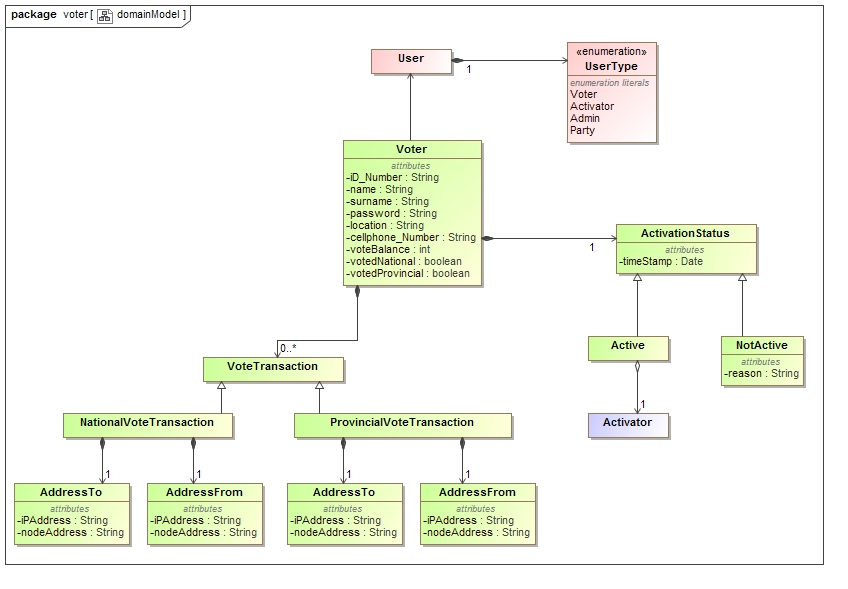
\includegraphics[width=0.75\linewidth]{../Images/DomainModels/voter_domainModel.png}
				\caption{Voter Domain Model}
			\end{figure}
			
			*insert discription here*
			\newline
			\item \textbf{Party}
			\begin{figure}[H]
				\centering
				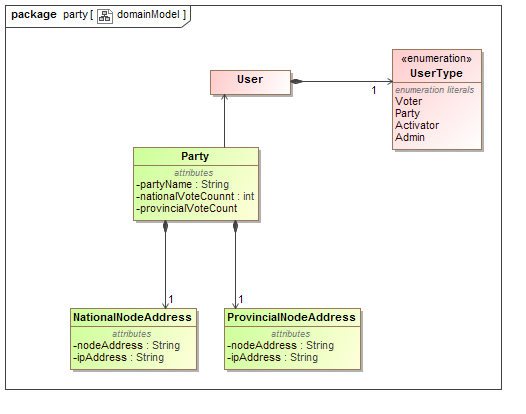
\includegraphics[width=0.75\linewidth]{../Images/DomainModels/party_domainModel.png}
				\caption{Party Domain Model}
			\end{figure}
			
			*insert discription here*
			\newline
			\item \textbf{Admin}
			\begin{figure}[H]
				\centering
				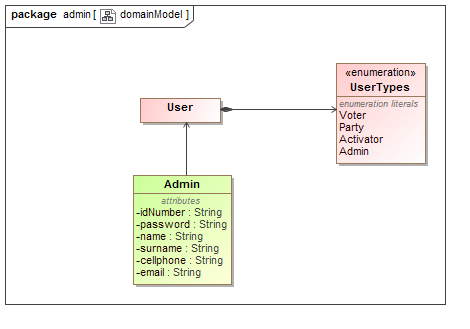
\includegraphics[width=0.75\linewidth]{../Images/DomainModels/admin_domainModel.png}
				\caption{Admin Domain Model}
			\end{figure}
			
			*insert discription here*
			\newline
			\item \textbf{Activator}
			\begin{figure}[H]
				\centering
				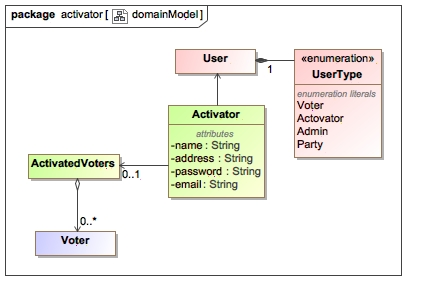
\includegraphics[width=0.75\linewidth]{../Images/DomainModels/activator_domainModel.png}
				\caption{Activator Domain Model}
			\end{figure}
			
			*insert discription here*
			\newline
\end{enumerate}
	
	\section{Open Issues}
		\subsection {GitHub Repository}
	\begin{enumerate}
		\item[] For more information and/or further references, please follow this \href{https://github.com/ish1993/eVoting}{link}, for access to Team CodeX's github repository.
	\end{enumerate}
	
\end{document}